\paragraph{Effect of radius}

For five different radii the maximum dynamic pressure and Mach number and the minimum height above Mars that were encountered on the first pass through the atmosphere were recorded. This is shown in figure \ref{fig:radius}. For each radius a trajectory for which the spacecraft just reaches the escape velocity (dark blue line, slow trajectory) and a trajectory which decelerates as fast as possible while staying under 3g deceleration (light blue line, fast trajectory) are calculated. These two orbits represent the two boundaries of what could possibly become the final orbit. In figure \ref{fig:radius} it can be seen that there is an approximately quadratic relationship between dynamic pressure and diameter for both limit orbits. It can also be seen that the fast trajectory has a higher dynamic pressure over the entire range of diameters. This is because the fast trajectory decelerates faster and goes deeper through the atmosphere. The minimal height achieved in the first pass is always 10 $\left[km\right]$ for the fast trajectory because in this trajectory the mission is terminated at 10 $\left[km\right]$ height within the first pass. For the slow trajectory it can be seen that a deeper pass through the atmosphere is needed with a lower diameter aeroshell. The same relation is true for the fast trajectory even though this can't be seen in this figure. The maximum Mach number encountered is constant for changing diameter and also for both limit orbits.
\begin{figure}[h]
	\centering
	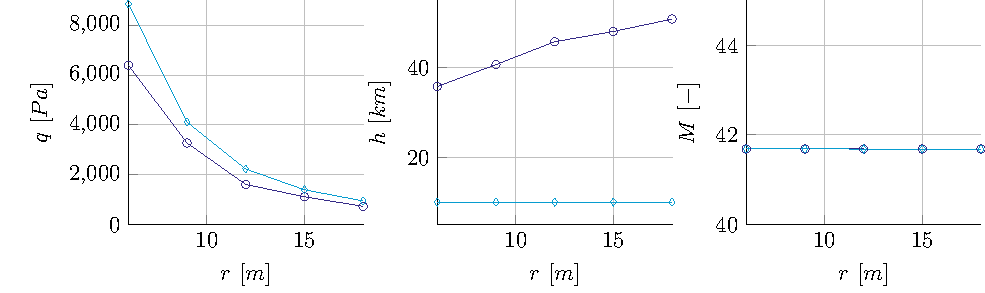
\includegraphics[width=\textwidth]{./Figure/orbit/radius_param.pdf}
	\caption{Maximum dynamic pressure, height and Mach number for different radii}
	\label{fig:radius}
\end{figure}


Apart from this results it should be noted that there is a lower limit to the diameter of the aeroshell imposed by the side heat flux into the capsule. For a large diameter the capsule is in the wake of the aeroshell and the side heat flux can thus be neglected. For a smaller diameter aeroshell eventually a backshell will be needed to protect the capsule. This will induce a unacceptable amount of mass.

\paragraph{Entry corridor}

The entry corridor is the fictional box where the re-entry vehicle should pass through to go into orbit. To low and the acceleration limit or the heat limit is breached, to high and the re-entry vehicle will skip on the atmosphere and never return. This corridor is dependent on different design parameters, the most important are the aerodynamic coefficients, entry velocity and control system.

**figure**

From a point in the middle of the entry corridor, as shown in figure \ref{fig:corridor}, the initial flight path angle (\gls{sym:gamma}), the angle of attack (\gls{sym:alpha}) and the bank angle (\gls{sym:mu}) have been changed to the utmost points where an orbit was still achieved. The effects of these changes separately are presented below.

\paragraph{Effect of initial flight path angle}

As can be seen in figure \ref{fig:effectgamma} the range of initial flight path angle for which an orbit is achieved is very limited. This means \gls{sym:gamma} has a big effect on the trajectory. For this small change in flight path angle the maximum dynamic pressure (\gls{sym:q}) increases by approximately $400 \left[Pa\right]$. It can also be seen the minimum height (\gls{sym:h}) decreases by more than two kilometers. The maximum Mach number (\gls{sym:M}) doesn't change for changing initial flight path angle.
\begin{figure}[h]
	\centering
	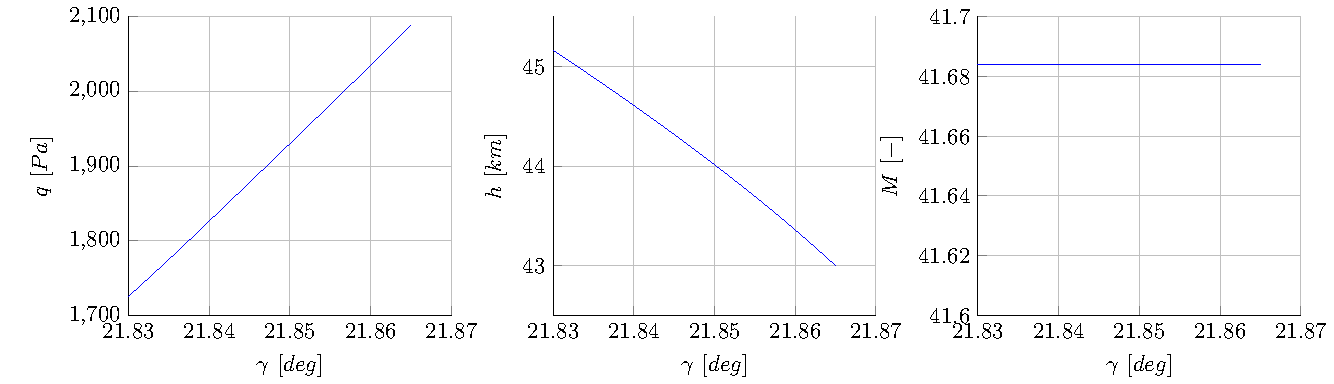
\includegraphics[width=\textwidth]{./Figure/orbit/effectgamma.pdf}
	\caption{Effect on dynamic pressure, height and Mach number for different flight path angles at $\gls{sym:alpha}=15 \left[deg\right]$ and $\gls{sym:mu}=30 \left[deg\right]$}
	\label{fig:effectgamma}
\end{figure}

\paragraph{Effect of angle of attack}

In figure \ref{fig:effectalpha} the range of angle of attack for which an orbit is achieved is shown. It can be observed that this window is five degrees wide. This means that the effect of \gls{sym:alpha} on the trajectory is significantly smaller than the effect of the flight path angle. However for this bigger change in angle still a big change both dynamic pressure (\gls{sym:q}) and height (\gls{sym:h}) is encountered. The maximum dynamic pressure increases by approximately $300 \left[Pa\right]$. It can also be seen the minimum height decreases by almost two kilometers. The maximum Mach number (\gls{sym:M}) doesn't change for changing angle of attack.
\begin{figure}[h]
	\centering
	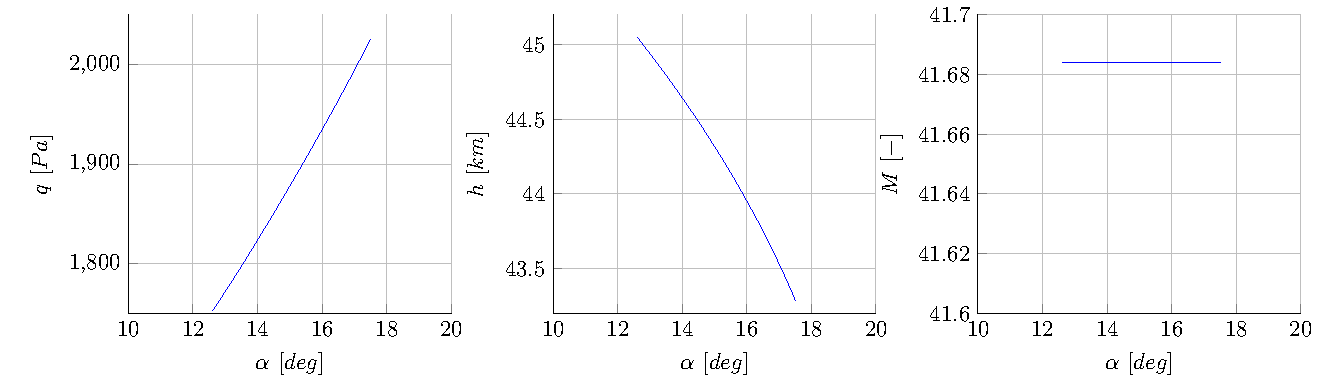
\includegraphics[width=\textwidth]{./Figure/orbit/effectalpha.pdf}
	\caption{Effect on dynamic pressure, height and Mach number for different angles of attack at $\gls{sym:gamma}=21.845 \left[deg\right]$ and $\gls{sym:mu}=30 \left[deg\right]$}
	\label{fig:effectalpha}
\end{figure}

\paragraph{Effect of bank angle}

As can be seen in figure \ref{fig:effectmu} the range for which an orbit is achieved changing only bank angle is almost $60 \left[deg\right]$. This means \gls{sym:mu} has to be changed a lot, compared to \gls{sym:gamma} and \gls{sym:alpha}, to have an effect on the orbit. This change in bank angle doesn't have a big effect on the maximum dynamic pressure (\gls{sym:q}) and the height (\gls{sym:h}). This indicates that the change in trajectory caused by a change in bank angle is much more subtle. The maximum Mach number (\gls{sym:M}) doesn't change for changing bank angle.
\begin{figure}[h]
	\centering
	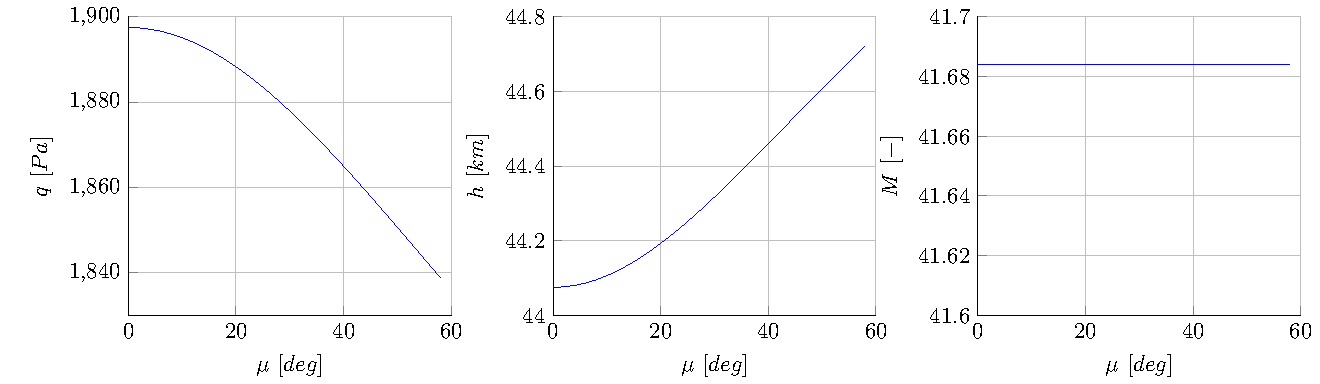
\includegraphics[width=\textwidth]{./Figure/orbit/effectmu.pdf}
	\caption{Effect on dynamic pressure, height and Mach number for different bank angles at $\gls{sym:alpha}=15 \left[deg\right]$ and $\gls{sym:gamma}=21.845 \left[deg\right]$}
	\label{fig:effectmu}
\end{figure}


